\section{Experiments}
\label{section:experiments}

In this section, we provide an empirical evaluation on our algorithms, verifying their
effectiveness on linearly separable datasets.
We generate strongly and weakly linearly separable datasets with $K=3$ classes in
$\R^3$, where the third dimension of every example is always equal to $1$
(i.e. a \emph{constant feature}).
See Figures~\ref{figure:strongly-separable-dataset} and~\ref{figure:weakly-separable-dataset}
 for visualizations
of the two datasets, along with detailed descriptions of the two data distributions.

%~\autoref{figure:strongly-and-weakly-separable-datasets}
%For both datasets, the sample size is $T=5\times 10^6$ and the
%margin is $\gamma=0.05$.
%Projections of the examples from the two datasets onto their first two coordinates
% are shown in
%We added a third dimension
%to every example that is equal to $1$. In other words, we added the so-called
%\emph{constant feature}. The constant feature is necessary so that
%\autoref{figure:strongly-separable-dataset} is actually strongly linearly
%separable.

\begin{figure}[h]
\centering
\begin{subfigure}[b]{0.23\textwidth}
\captionsetup{justification=centering}
\begin{center}
\hspace*{-0.3cm} 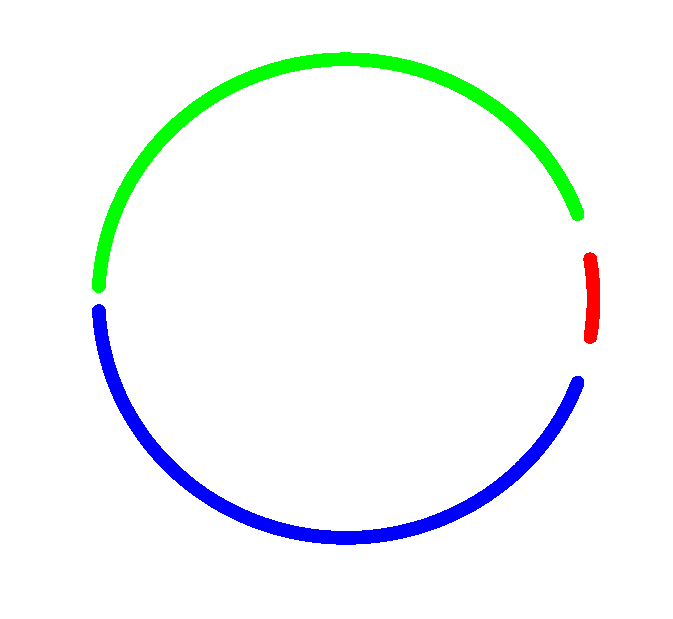
\includegraphics[width=1.15\textwidth, trim={0, 0cm, 0, 0}, clip]{figures/strong_points}
\caption{Strongly separable case}
\label{figure:strongly-separable-dataset}
\end{center}
\end{subfigure}
\hfill
\begin{subfigure}[b]{0.23\textwidth}
\captionsetup{justification=centering}
\centering
\hspace*{-0.3cm}  \includegraphics[width=1.15\textwidth, trim={0, 0cm, 0, 0}, clip]{figures/weak_points}
\caption{Weakly separable case}
\label{figure:weakly-separable-dataset}
\end{subfigure}
\vspace*{-0.2cm}
\caption{Strongly and weakly separable datasets with $K=3$ classes. Here
 we show projections of the examples onto their first two coordinates, which
 lie in the unit ball of $\R^2$. Class 1 is depicted red. Classes 2 and
3 are depicted green and blue, respectively. $80\%$ of the examples belong to class 1,
$10\%$ belong to class 2 and $10\%$ belong to class 3. Class 1
occupies the angle interval $[-15^\circ, 15^\circ]$, while classes 2 and 3
occupy angle intervals $[15^\circ, 180^\circ]$ and $[-180^\circ, -15^\circ]$
respectively. The examples are strongly and weakly linearly separable with a margin of $\gamma=0.05$, respectively.}
\label{figure:strongly-and-weakly-separable-datasets}
\end{figure}

%We removed points that lie within margin $\gamma=0.05$ of the
%linear separator.

We implement
Algorithm~\ref{algorithm:algorithm-for-strongly-linearly-separable-examples},
Algorithm~\ref{algorithm:kernelized} with
rational kernel~\eqref{equation:rational-kernel}, and the \textsc{Banditron} algorithm.
We evaluate these algorithms on the above two datasets, with a time horizon of
$T=5\times 10^6$.
\textsc{Banditron}
has exploration rate parameter $\epsilon$, for which we tried values $\epsilon
\in \{0.02, 0.01, 0.005, 0.002, 0.001, 0.0005 \}$.
Since all three
algorithms are randomized, we run each algorithm $20$ times.
The average cumulative number
of mistakes up to round $t$ as a function of $t$ are shown in
Figures~\ref{figure:number-of-mistakes-strongly-separable-dataset}
and~\ref{figure:number-of-mistakes-weakly-separable-dataset}.

We can see that there is a tradeoff in the setting of the exploration rate $\epsilon$
for \textsc{Banditron}. For a large $\epsilon$, \textsc{Banditron} suffers from the cost of exploration, whereas for small $\epsilon$, its model cannot be updated quickly enough.
As expected, Algorithm~\ref{algorithm:algorithm-for-strongly-linearly-separable-examples} has a small number of mistakes in the strongly linearly separable setting, while having a large number
of mistakes in the weakly linearly separable setting, due to the limited representation power of linear classifiers.
In contrast,
Algorithm~\ref{algorithm:kernelized} with rational kernel has a small number of mistakes in both settings, exhibiting strong adaptivity guarantees. Appendix~\ref{section:supp-to-experiment} shows the decision boundaries
that each of the algorithms learns.

%This problem is exacerbated when a class of large proportion occupies a small region
%(e.g. class 1).
%In contrast, our algorithms make
%significant progress on every mistake it makes, leading to a finite mistake
%bound.
%Striking a balance between the two extremes leads to the
%$\Theta(\sqrt{T})$ number of mistakes.

\begin{figure}
\centering
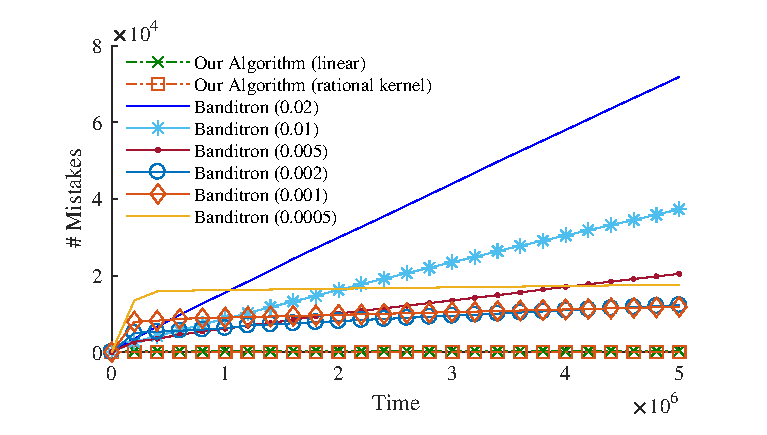
\includegraphics[width=0.45\textwidth]{figures/strong3}
\caption{The cumulative number of mistakes versus the number of rounds,
in the strongly separable case (\autoref{figure:strongly-separable-dataset}) for various algorithms.}
\label{figure:number-of-mistakes-strongly-separable-dataset}
\end{figure}

\begin{figure}
\centering
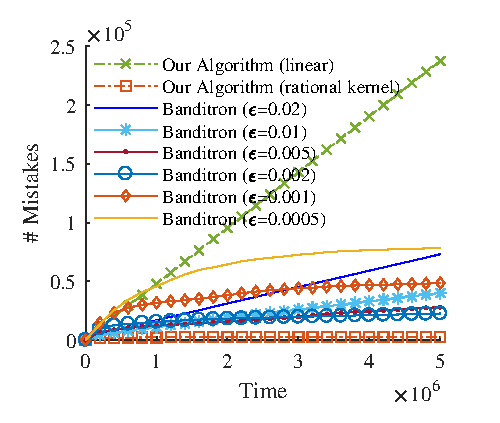
\includegraphics[width=0.45\textwidth]{figures/weak3}
\caption{The cumulative number of mistakes versus the number of rounds,
in the weakly separable case (\autoref{figure:weakly-separable-dataset}) for various algorithms.}
\label{figure:number-of-mistakes-weakly-separable-dataset}
\end{figure}
